% Adapted from Alex Reustle's CMSC351 Course Notes

% This program is free software: you can redistribute it and/or modify
% it under the terms of the GNU General Public License as published by
% the Free Software Foundation, either version 3 of the License, or
% (at your option) any later version.

% This program is distributed in the hope that it will be useful,
% but WITHOUT ANY WARRANTY; without even the implied warranty of
% MERCHANTABILITY or FITNESS FOR A PARTICULAR PURPOSE.  See the
% GNU General Public License for more details.

% You should have received a copy of the GNU General Public License
% along with this program.  If not, see <http://www.gnu.org/licenses/>.
\documentclass[english, 10pt]{article}

\usepackage{notes}
\usepackage{inconsolata}
\usepackage[shellescape]{gmp}
\allowdisplaybreaks%
\newcommand{\thiscoursecode}{CMSC 320}
\newcommand{\thiscoursename}{Introduction to Data Science}
\newcommand{\thisprof}{Prof.\ John Dickerson}
\newcommand{\me}{Akilesh Praveen}
\newcommand{\thisterm}{Fall 2020}
\newcommand{\website}{https://cmsc320.github.io}%chktex 8
\usepackage{ifpdf}
\ifpdf%
\DeclareGraphicsRule{*}{mps}{*}{}
\fi
% \listfiles

\usepackage[utf8]{inputenc}
 
\usepackage{listings}
\usepackage{xcolor}
\usetikzlibrary{patterns}
 
\definecolor{codegreen}{rgb}{0,0.6,0}
\definecolor{codegray}{rgb}{0.5,0.5,0.5}
\definecolor{codepurple}{rgb}{0.58,0,0.82}
\definecolor{backcolour}{rgb}{0.95,0.95,0.94}
\definecolor{codered}{rgb}{0.5,0.15,0.15}
\definecolor{commentred}{rgb}{1,0.01,0.02}
 
\lstdefinestyle{mystyle}{
    backgroundcolor=\color{backcolour},   
    commentstyle=\color{codegreen},
    keywordstyle=\color{red},
    numberstyle=\tiny\color{codegray},
    stringstyle=\color{codered},
    basicstyle=\ttfamily\footnotesize,
    breakatwhitespace=false,         
    breaklines=true,                 
    captionpos=b,                    
    keepspaces=true,
    xleftmargin=.15\textwidth,
    xrightmargin=.15\textwidth,
    linewidth=\textwidth,                 
    numbers=left,                    
    numbersep=5pt,                  
    showspaces=false,                
    showstringspaces=false,
    showtabs=false,                  
    tabsize=2,
    belowskip=3em,
    aboveskip=3em,
}

\lstset{style=mystyle}


% \VerbEnvir{align tikzpicture algorithm}
%%%Headers
\chead{320 - Intro to Data Science}
\lhead{\thisterm}

%%%%% TITLE %%%%%
\graphicspath{{../}}
\newcommand{\notefront}{%
\pagenumbering{arabic}
\begin{center}
{\small}
\textbf{\Huge{\noun{\thiscoursecode}}}
{\Huge \par}
{\Large{\noun{\thiscoursename}}}\\
\vspace{0.1in}
\vspace{0in}
\includegraphics[scale=0.3]{umd_cs.jpg} \\
\vspace{0.1in}{\noun\me} \\
{\noun\thisprof} \ $\bullet$ \ {\noun\thisterm} \ $\bullet$ \ {\noun{University of Maryland}} \\
{\ttfamily \url{\website}} \\
\end{center}
}

 \tikzstyle{class}=[
    rectangle,
    draw=black,
    text centered,
    anchor=north,
    text=black,
    text width=2cm,
    shading=axis,
    bottom color={rgb:red,222;green,222;blue,222},
    top color=white,shading angle=45]

\begin{document}
% \renewcommand\familydefault{\sfdefault}
% \sffamily
  % Notes front
  \notefront%
  % Table of Contents and List of Figures
  \tocandfigures%
  
\section{Notes \& Preface}

Course notes for CMSC320, under Prof. John Dickerson. Notes collected from previous and current lectures.

\section{Lecture 1}

\subsection{What is Data Science?}

Data Science is the application of computation and statistical techniques to address or gain insight.
It's the intersection of statistics and Computer Science.
Based on what I've learned thus far, learning to do data science is like learning how to use a TI-84 in statistics class.
You're simply learning how to leverage programming tools in order to perform advanced, complex, and meaningful data-related operations.\newline

It's the use of statistics and computer science in order to find real-world insights.\newline\newline

{
\centering


\tikzset{every picture/.style={line width=0.75pt}} %set default line width to 0.75pt        

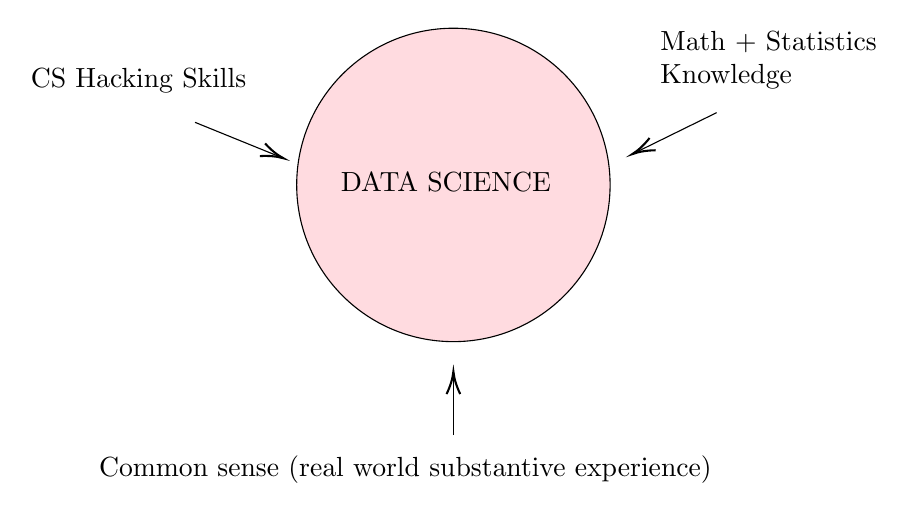
\begin{tikzpicture}[x=0.75pt,y=0.75pt,yscale=-1,xscale=1]
%uncomment if require: \path (0,300); %set diagram left start at 0, and has height of 300

%Shape: Circle [id:dp061140258122834745] 
\draw  [fill={rgb, 255:red, 255; green, 219; blue, 224 }  ,fill opacity=1 ] (254.67,119.5) .. controls (254.67,77.8) and (288.47,44) .. (330.17,44) .. controls (371.86,44) and (405.67,77.8) .. (405.67,119.5) .. controls (405.67,161.2) and (371.86,195) .. (330.17,195) .. controls (288.47,195) and (254.67,161.2) .. (254.67,119.5) -- cycle ;
%Straight Lines [id:da4450208385410075] 
\draw    (205.67,89.33) -- (246.48,105.91) ;
\draw [shift={(248.33,106.67)}, rotate = 202.11] [color={rgb, 255:red, 0; green, 0; blue, 0 }  ][line width=0.75]    (10.93,-3.29) .. controls (6.95,-1.4) and (3.31,-0.3) .. (0,0) .. controls (3.31,0.3) and (6.95,1.4) .. (10.93,3.29)   ;
%Straight Lines [id:da055339322100053545] 
\draw    (457,84.67) -- (418.13,103.78) ;
\draw [shift={(416.33,104.67)}, rotate = 333.81] [color={rgb, 255:red, 0; green, 0; blue, 0 }  ][line width=0.75]    (10.93,-3.29) .. controls (6.95,-1.4) and (3.31,-0.3) .. (0,0) .. controls (3.31,0.3) and (6.95,1.4) .. (10.93,3.29)   ;
%Straight Lines [id:da5012858238681945] 
\draw    (330.17,240) -- (330.17,211.33) ;
\draw [shift={(330.17,209.33)}, rotate = 450] [color={rgb, 255:red, 0; green, 0; blue, 0 }  ][line width=0.75]    (10.93,-3.29) .. controls (6.95,-1.4) and (3.31,-0.3) .. (0,0) .. controls (3.31,0.3) and (6.95,1.4) .. (10.93,3.29)   ;

% Text Node
\draw (274.67,112.5) node [anchor=north west][inner sep=0.75pt]   [align=left] {DATA SCIENCE};
% Text Node
\draw (125.33,62) node [anchor=north west][inner sep=0.75pt]   [align=left] {CS Hacking Skills};
% Text Node
\draw (428.67,44.33) node [anchor=north west][inner sep=0.75pt]   [align=left] {Math + Statistics\\Knowledge};
% Text Node
\draw (158.17,248.67) node [anchor=north west][inner sep=0.75pt]   [align=left] {Common sense (real world substantive experience)};


\end{tikzpicture}

}

\subsection{Topics}

Here are the general topics that this class will cover.

\begin{itemize}
	\item Processing data
	\item Visualizing data
	\item Understanding data
	\item Communicating data
	\item Extracting value from data
\end{itemize}

\subsection{Tools}

Here are some tools commonly employed by data scientists. We'll try to cover how to use most of them here.

\begin{itemize}
	\item Python
	\item Scikit-Learn
	\item Docker
	\item PANDAS
	\item Spark
	\item TensorFlow
\end{itemize}

\subsection{Conda}

Conda is a package and environment manager for python that we can use with the command line.
We can create multiple environments for us and install separate packages in each of them.
This will be highly useful to us, as we sometimes want to consolidate the tools we use into separate environments.

\section{Test Section}

\subsection{Lower Level}

Here's a cool code example.

{\centering
\begin{lstlisting}[language=C]
#include <stdio.h>
#include <math.h>

int main() {
   double value;

   printf("Enter a number: ");
   scanf("%lf", &value);     /* Notice the use of %lf */

   printf("sqrt %f: \n", sqrt(value));
   printf("power of 2: %f\n", pow(value, 2));
   printf("sin: %f\n", sin(value));

   return 0;
}
\end{lstlisting}
}

Here's some more information about our code example.



\section{Footnotes}

Taken by Akilesh Praveen.

\end{document}
